\section{Analysis}
\label{sec:analysis}
%(2 pages)

As noted previously, progress on knowledge base population has been slow and arduous \pl{cite?}.
Let's proceed with an analysis of submissions and evaluations thus far, with the motivation of identifying potential obstacles for system development. 

\paragraph{Data.}
We will make use of system submissions released as part of the TAC-KBP Slot Validation tracks in 2013, 2014 and 2015.
The 2015 dataset contains 70 submissions from 18 teams for 317 queries.
Considering only the submissions to the first hop of the two-hop \pl{to non-KBP person, don't know what this means} evaluation,
each submission contains on average about 35,951 predicted slotfills. 
There are in total 201,332 relations that were predicted, of which only 11,008 of these slotfills have were evaluated.

\subsection{What is the effect of pooling?}

\begin{figure*}
  \begin{subfigure}{\columnwidth}
  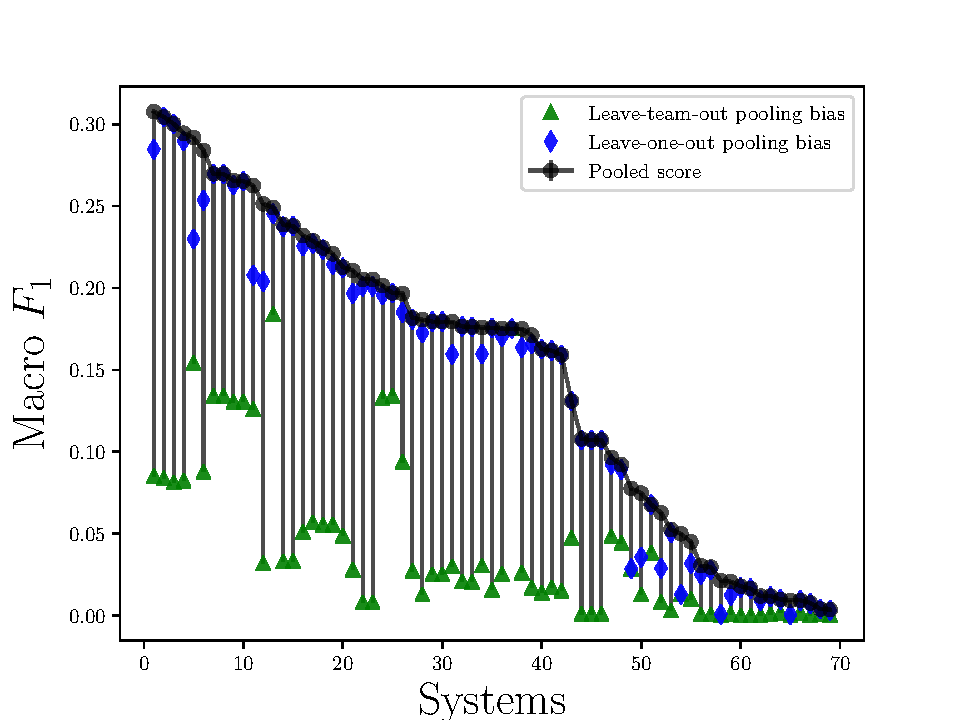
\includegraphics[width=\columnwidth]{figures/pooling-bias}
  \caption{\label{fig:pooling-bias} Pooling bias for the macro \fone{} metric.}
  \end{subfigure}
  \begin{subfigure}{\columnwidth}
  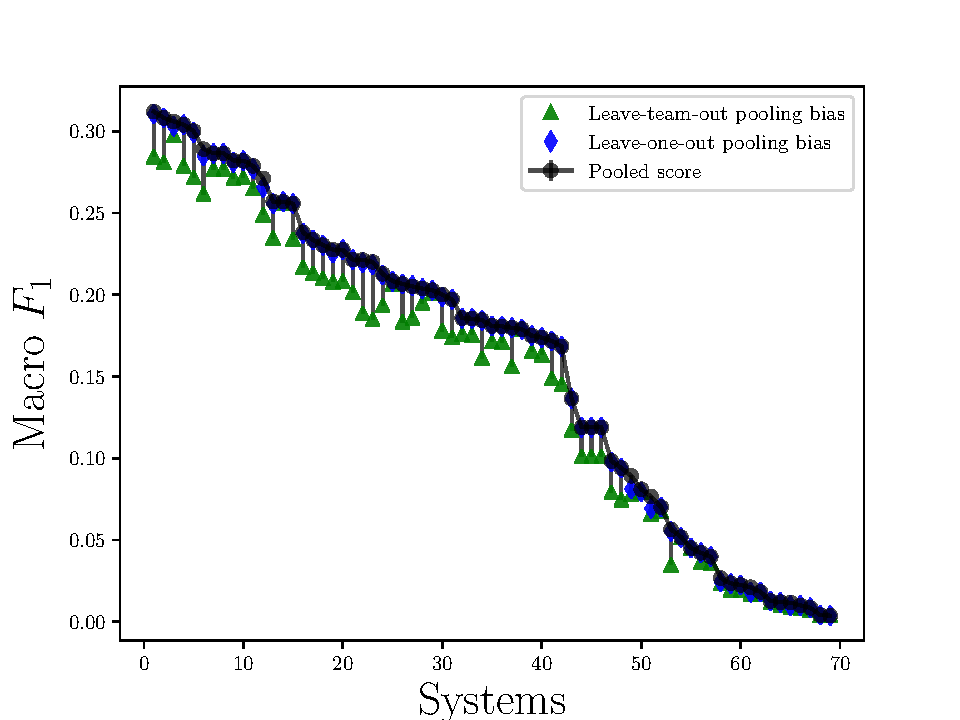
\includegraphics[width=\columnwidth]{figures/pooling-bias-anydoc}
  \caption{\label{fig:pooling-bias-anydoc} Pooling bias for the macro \fone{} metric with the `anydoc' heuristic.}
  \end{subfigure}
  \caption{Pooling bias measures how much a system's score is affected by not having its output as part of the pooled evaluation.
  The median bias on the top 40 teams against an unpooled team is 15.51\% points for the standard macro \fone{} metric and 1.98\% when evaluating using the anydoc heuristic.
  Note that the median difference between the anydoc scores and standard scores is 0.74\% points; this difference is caused because the anydoc heuristic erroneously scores fills with incorrect judgements to be correct.}
\end{figure*}

The ``gold'' labels on relation contexts are collected by a combination of a time-bounded human search in the corpus and a human evaluation of pooled output from participating systems.
While the human search identifies a significant fraction of relations (\todo{80\%}),
  it does not sufficiently cover the variety of contexts that are submitted as justifications of the relation. 
This has two implications on how a development system, \textit{D}, that did not participate in the original evaluation is scored.
Firstly, it is likely that contexts \pl{I thought the problem with bias was due to the set of relations $D$ returns, not contexts} the system \textit{D} submits has never been seen before and hence can not be evaluated.
Secondly, it is also likely that relations the system \textit{D} submits have never been seen before, particularly if \textit{D} incorporates a novel method of relation extraction, creating a perverse incentive to ensure that new extraction methods behave similarly to old extraction systems.
The magnitude of this effect, the pooling bias, is can be quantified by performing a ``leave-one-out'' (``leave-team-out'') experiment on previous years submissions, measuring the difference in metric scores when output unique to a single submission (team) is excluded from the gold data.
The former is a proxy that measures how much bias development systems of teams that had participated in the KBP evaluation experience and the latter measures the bias development systems of new teams experience.
\figureref{pooling-bias} shows the pooling bias experienced by teams and systems in the 2015 evaluation;
  the median bias against an unpooled team is 13.55\% \fone{} points and for an unpooled system is 4.55\% \fone{} points,
  making it impossible to evaluate against this metric in development (also significantly biasing new entrants to the task).

To mitigate this unreasonable bias, teams typically adopt an `anydoc' heuristic during evaluation, which ignores the justification of a context while evaluating a relation.
\pl{hard for me to get intuition for implications of anydoc}
With this heuristic (\figureref{pooling-bias-anydoc}), the pooling bias decreases considerably, with 
  the median bias against an unpooled team being 1.98\% \fone{} points and unpooled system is 0.0\% \fone{} points.
However, it should also be noted that scores under the `anydoc' heuristics are on average 0.74\% higher than the standard scores due to erroneously labeling entries to be correct.
This analysis confirms the necessity of the `anydoc' heuristic on the current evaluations, but regardless, the bias is large enough to wash out the effect of the typical improvement a development makes.
% TAKEAWAY: new entrants are biased against!

In the latter sections of this paper, we eliminate the problem of pooling evaluation all together by proposing an online evaluation methodology where every new submission is considered and selectively evaluated to ensure statistical validity.

% NOTE: should we describe any more statistics?
\paragraph{How informative is \fone{} as a metric?}
\ac{Ignore for now!}
\begin{figure*}
  \begin{subfigure}{0.49\textwidth}
  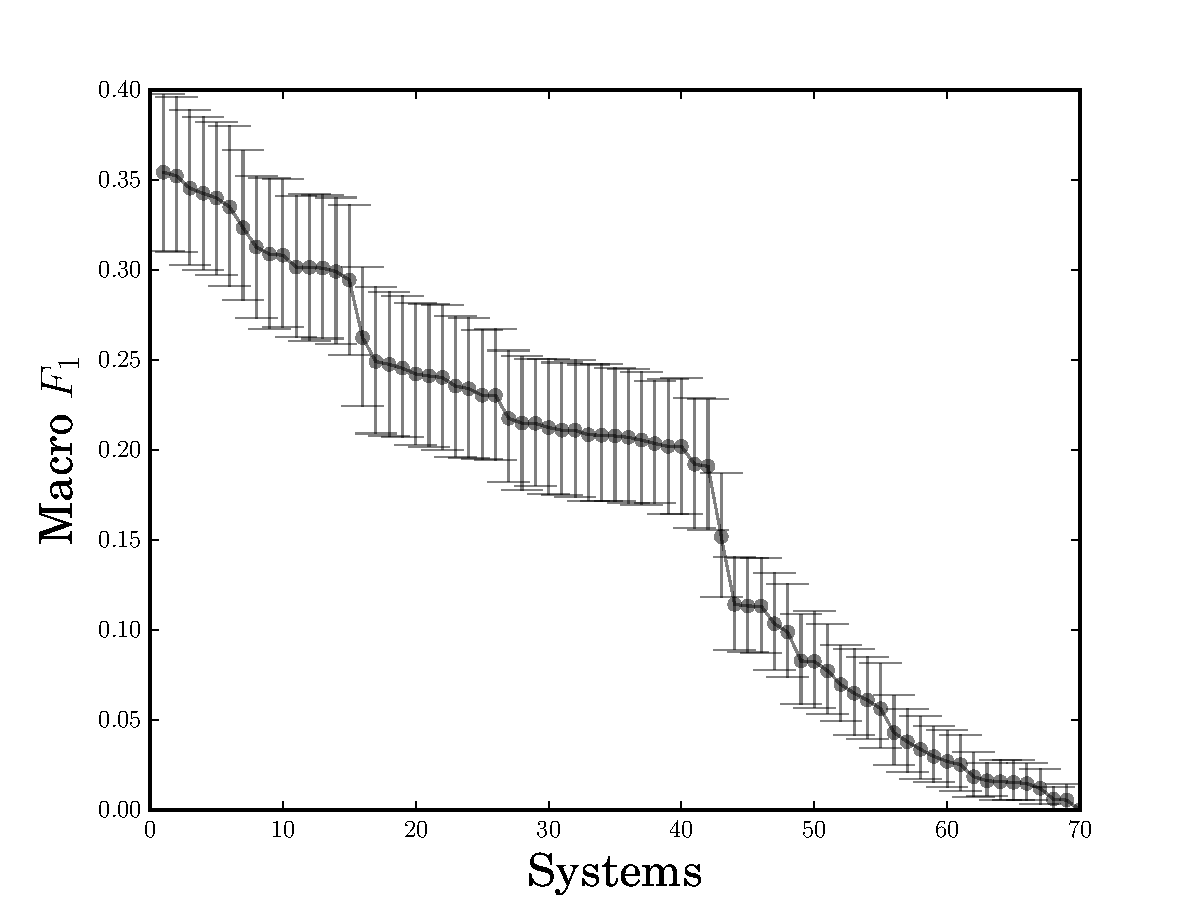
\includegraphics[width=\columnwidth]{figures/experiment1}
  \caption{\label{fig:f1}}
  \end{subfigure}
  \begin{subfigure}{0.49\textwidth}
  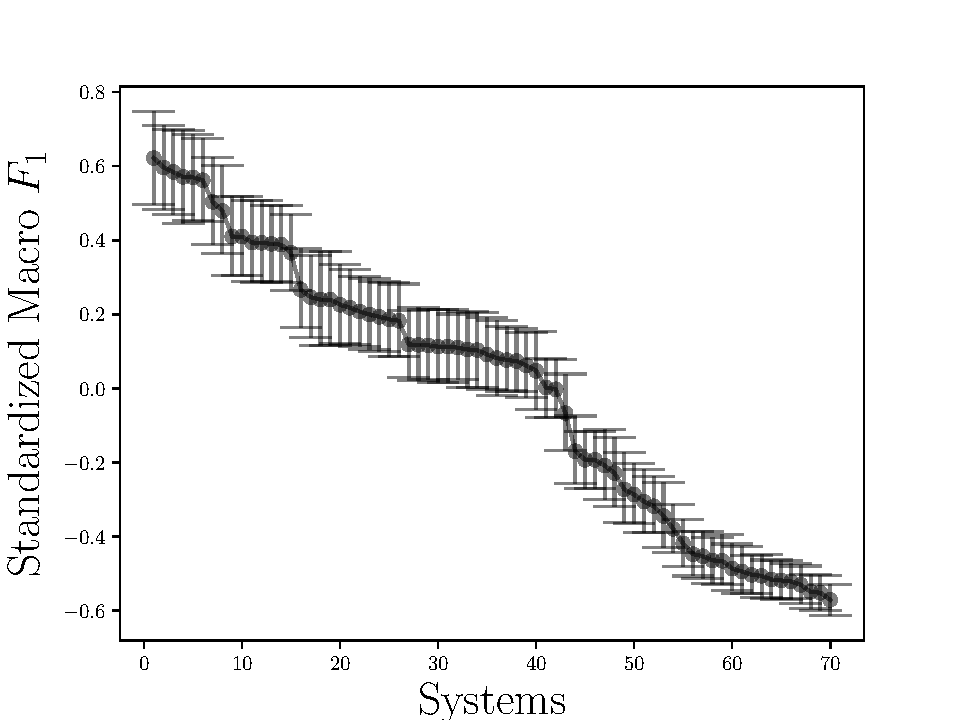
\includegraphics[width=\columnwidth]{figures/experiment3}
  \caption{\label{fig:sf1}}
  \end{subfigure}
  \caption{}
\end{figure*}

\begin{table*}
  \begin{tabular} {l r r r r r} \toprule
    Metric & \multicolumn{3}{c}{Normal} & \multicolumn{2}{c}{Standardized} \\
           & Average value & 95\% confidence interval & Mean difference between top 10 teams &  Average value & 95\% confidence interval  \\  \midrule 
Micro $P^e$     & $30.91\%$ &  $16.77\%$ & 0.12\% &     &  \\
Micro $R^e$     & $30.45\%$ &  $ 6.41\%$ & 0.17\% &     &  \\
Micro $\fone^e$ & $38.62\%$ &  $ 6.79\%$ & 0.24\% &     &  \\
Macro $P^e$     & $24.98\%$ &  $ 6.93\%$ & 0.24\% &     &  \\
Macro $R^e$     & $03.56\%$ &  $ 6.87\%$ & 0.23\% &     &  \\
Macro $\fone^e$ & $22.72\%$ &  $ 6.19\%$ & 1.04\% &     &  \\ \bottomrule
  \end{tabular}

\begin{tabular}{l r r r r r} \toprule
  Metric ($\sigma^2$) & System variance ($\sigma^2_{s}) $ & Query variance($\sigma_{e}$) & Residual ($\sigma_{s,e})$ \\ \midrule % & $\psi$  & $\rho$ \\
  \fone{} (0.102) & 11.75\% & 20.59\% & 66.66\% \\ \bottomrule % &     0.120 & 0.152
\end{tabular}
  \caption{\label{metric-variance}}
\end{table*}

Most teams hill climb on a combination of micro and macro entity-level $\fone$ during development.
It is natural to ask how much of an improvement on the metric score is necessary to actually trust that system performance has improved.
We use a bootstrap sampling \pl{what exactly is being resampled?} method to estimate the variance of $\fone$ and other metrics over query sets \tableref{metric-variance} and measure the 95\% confidence intervals for system scores \figureref{f1}.
The median difference in metric scores between adjacent submissions in the top 10 scores (for that metric) is between 0.1--1\%,
while the confidence intervals are at least 6\%.
% TODO: we can use the differences between the submissions of the each team.
It is hard for the researcher to identify if any of the presumably distinct submissions hold any water of another. \pl{awkward}

Next, we would like to ask what factors contribute to the large variance in the system metrics above.
One natural confounding variable is the substantial variability in the difficulty of query entities.
We can measure the effect of the query entity by analyzing the variation in topic-model scores.
Consider the linear model, \pl{$\mu$'s don't cancel out}
\begin{align*}
  X_{s,e} &= \mu 
    + \underbrace{\mu_{s} - \mu}_{\nu_{s}}
    + \underbrace{\mu_{e} - \mu}_{\nu_{e}}
    + \underbrace{X_{s,e} - \nu_{s} - \nu_{e} - \mu}_{\nu_{s,e}},
\end{align*}
where $\nu_{s}$, $\nu_{e}$ and $\nu_{s,e}$ capture the effect of the system $s$ and query entity $e$, and the residual.
Variance can also be decomposed as,
\begin{align*}
  \sigma^2(X_{s,e}) &= \sigma^2(\nu_s) + \sigma^2(\nu_e) + \sigma^2(\nu_{s,e}).
\end{align*}

\tableref{} shows the variance explained by different components for macro metrics. As we can see, almost twice as much of the variance is explained by the entity only as that of the system.
\pl{this is true of any task in general, right, not just KBP?  easy examples everyone gets,
hard examples, some people get?}
% Explain what the high q,e scores mean.
%Another consequence is in confidence intervals.
%Bad differentiation from pairwise scores.

% TODO: replace with a GLMM

\paragraph{Controlling for query variance.}
\ac{Ignore for now!}

It's easy for us to control for query variance by standardizing our metric,  
$$X'_{se} = \frac{X_{se} - \mu_e}{\sigma_e}$$.

\figureref{sf1} plots the performance of systems under the standardized macro \fone metric.
% TODO: variance under standardized metric -- showing less contribution
% due to queries and an overall reduction in variance.
% NOTE: This is only useful when comparing systems, as one is wont to do during development.

% TODO: I wish we could give scroes for this.
% \subsection{Are we improving over time?}

